\section{Run-time View}
These sequence diagrams show how the different components of the system interact with each other.

\subsection{Login}
A Third Party goes to the login Web page of the TrackMe Web application to be authenticated, in order to be able to use the services provided by the TrackMe system. It inserts its credentials (username and password). The Request Module checks if the inserted data match with an existent account. If the Third Party is recognized, it is logged into the system.

\begin{figure}[H]

    \centering
    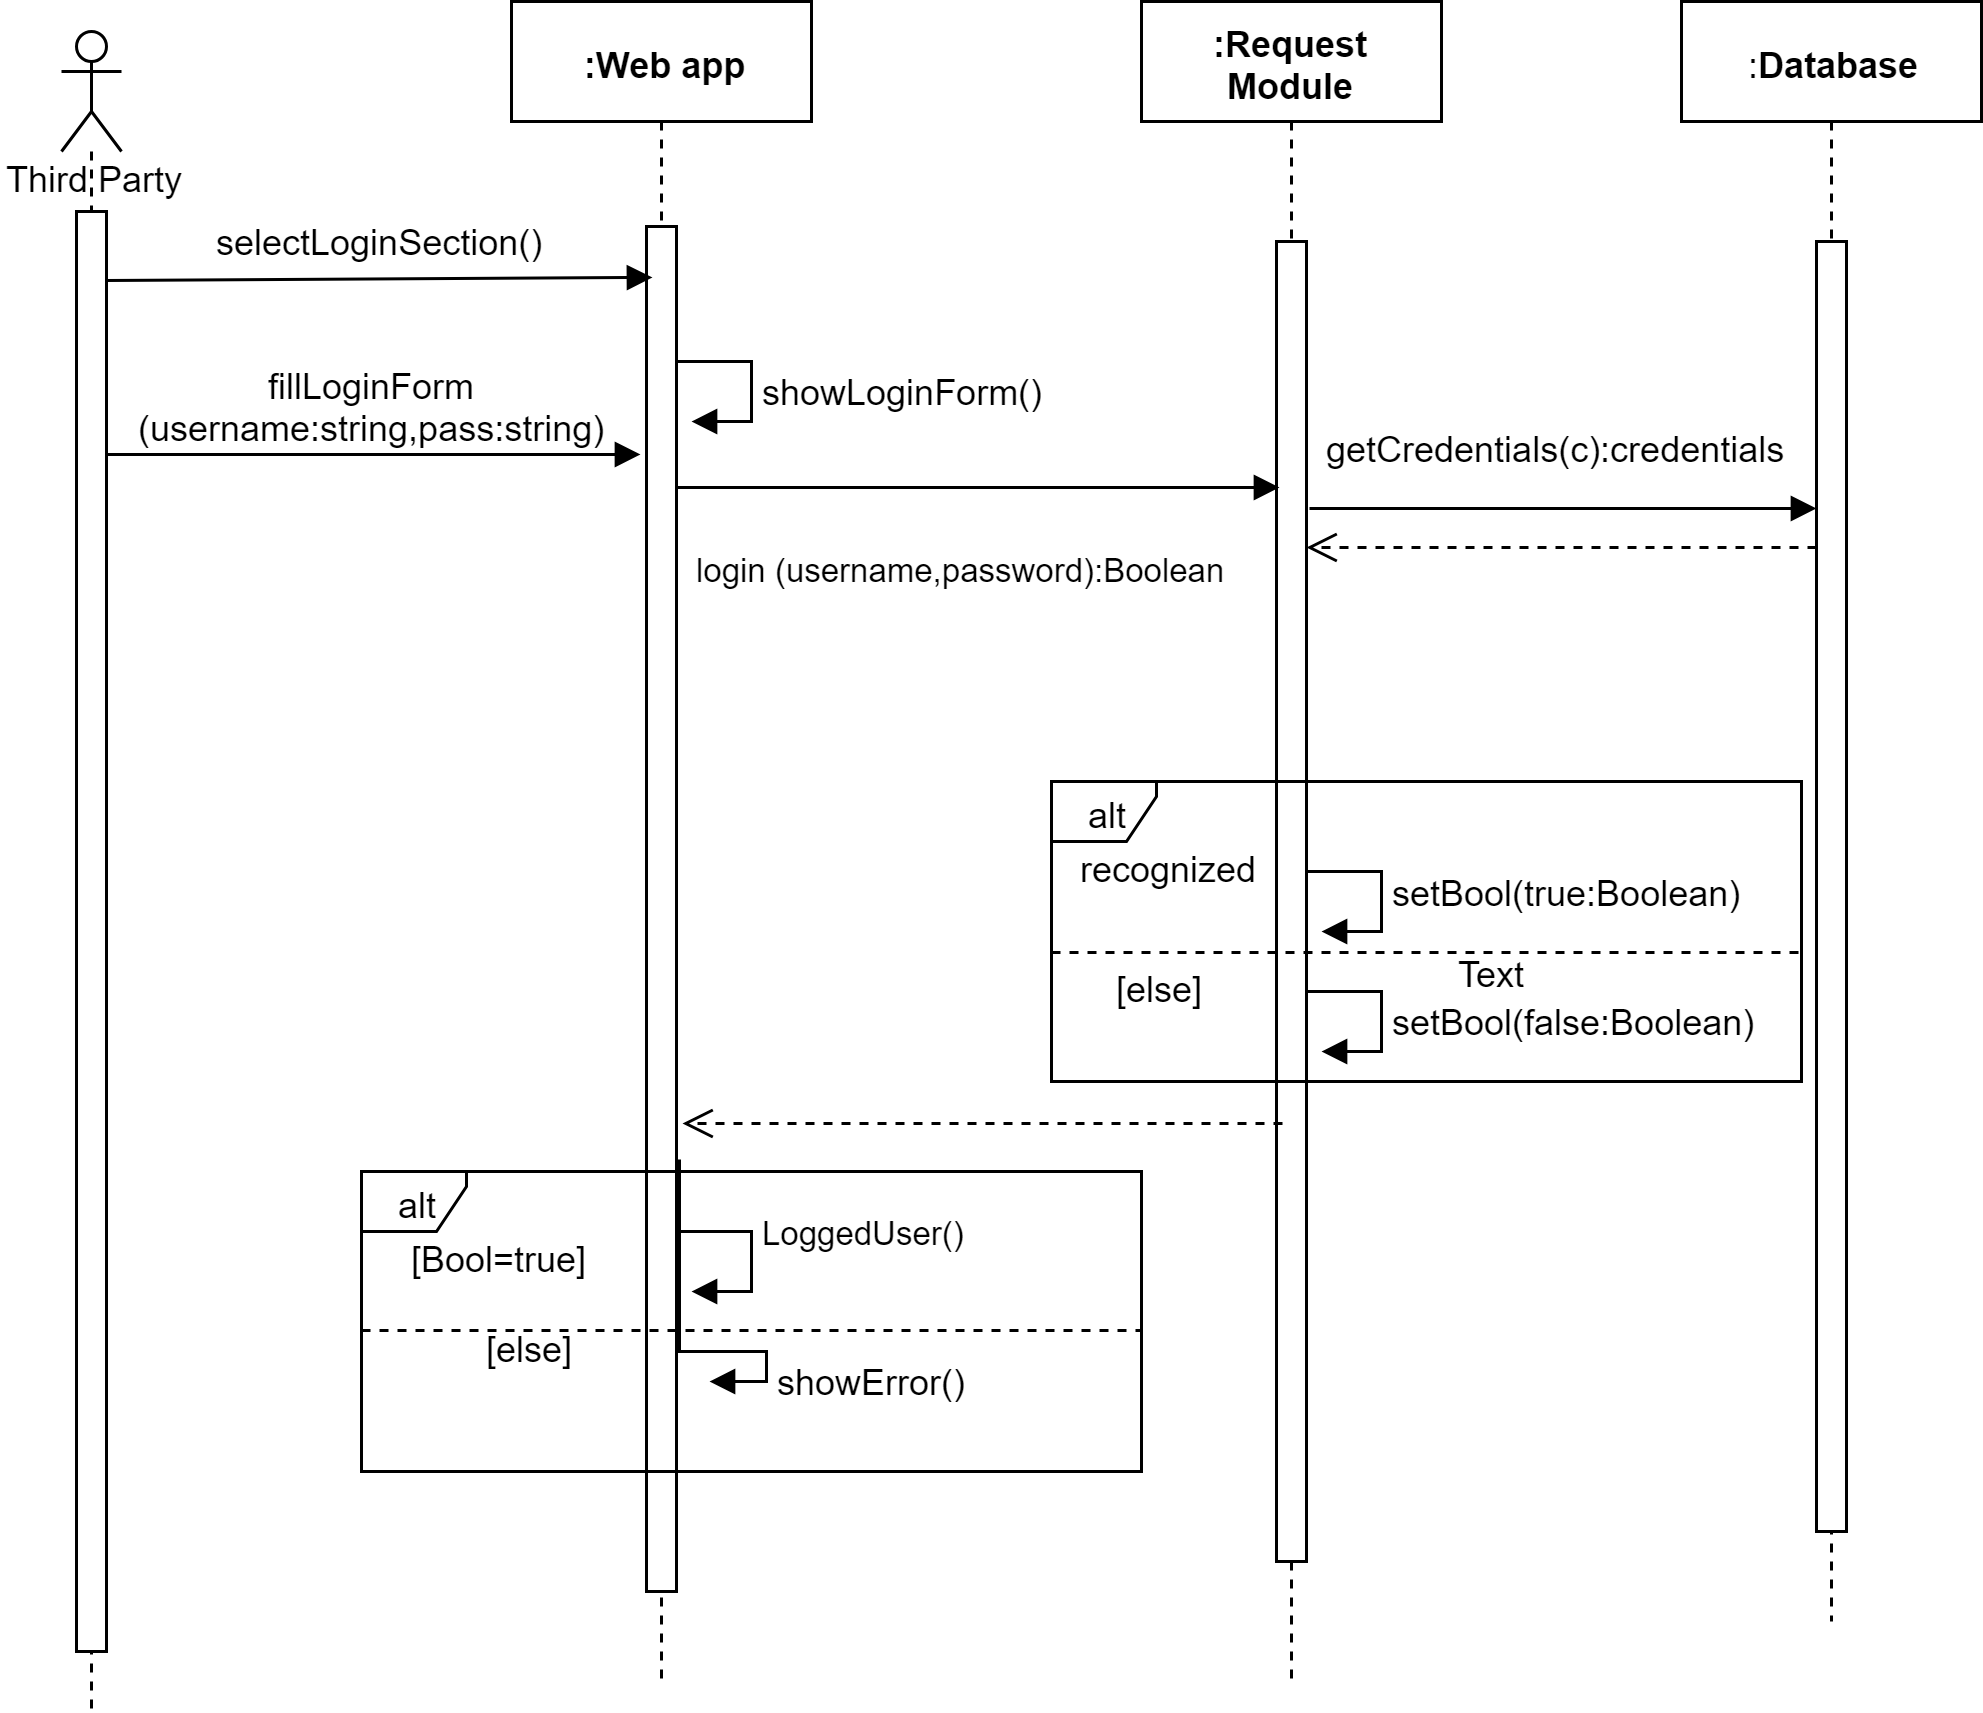
\includegraphics[scale=0.15]{./Pictures/login.png}
    \caption{Login sequence diagram}
    
\end{figure}

The Login process for a User of the Mobile application is the same.\\ \\
From now on we consider that the Users are logged into the system.

\subsection{Dispatch of a User subscription request}
A Third Party selects the New Request button in the individuals section with subscription mode; the Third Party fills out the form with the fiscal code of the target individual, the data that it wants to receive (this selection is permitted by the use of boolean values) and an interval time corresponding to the desired update frequency. The Request Module creates a new request with the selected data and stores it in the database. After that, the module notifies the target User that there is a new request to manage in his/her incoming request section.

\begin{figure}[H]

    \centering
    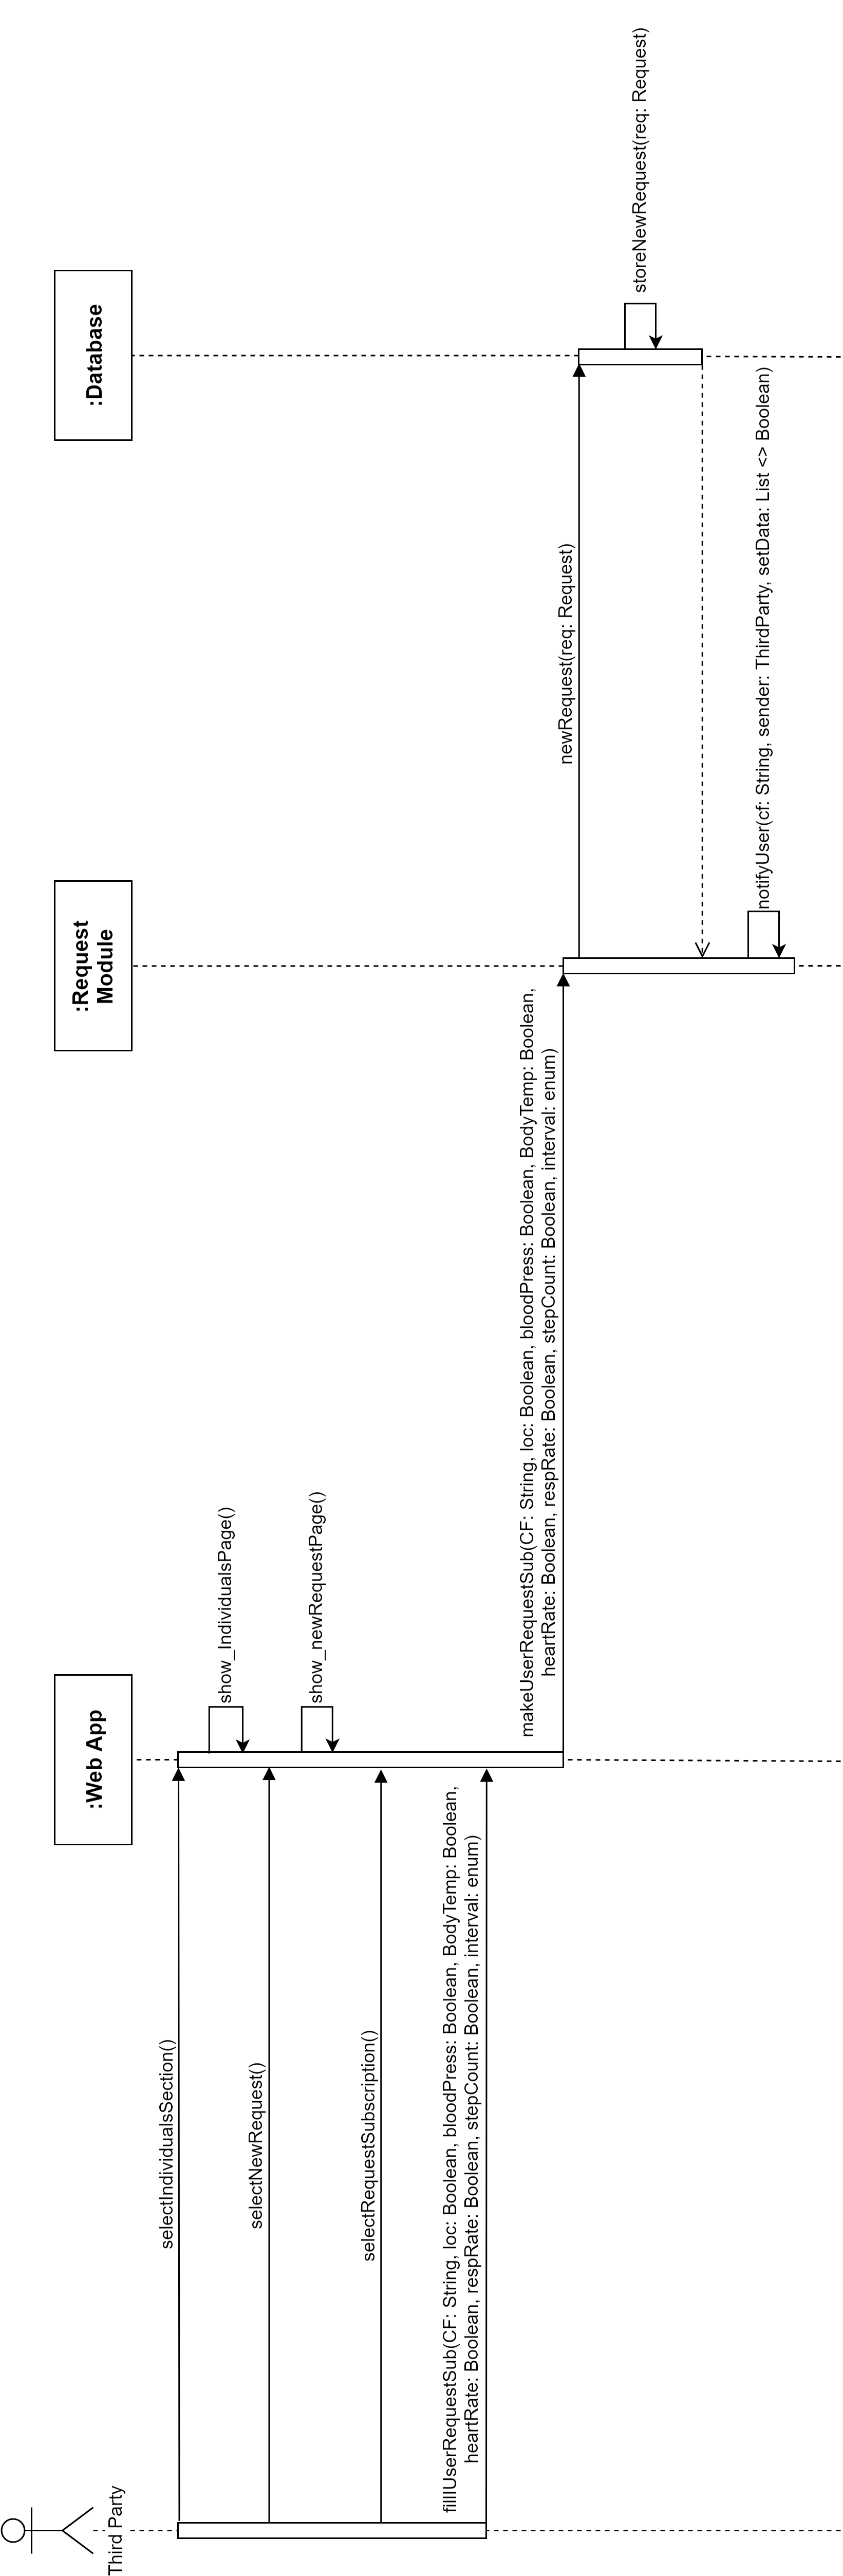
\includegraphics[scale=0.16]{./Pictures/userRequestV.png}
    \caption{User request by a Third Party}
    
\end{figure}

\subsection{Manage of incoming User Requests}
A User can manage incoming requests by clicking on the appropriate section. The Manage Request Module queries the database for the list of requests that the User has received and shows it. The User can select a specific request and the application shows all the details:
the name of the Third Party which performed the request, the list of data in which it is interested in, the selected update interval time. At this point the User can decide to accept or deny the request; the Manage Request Module stores the response in the database, updating the status of the request. Finally, it notifies the request sender, informing it that the request is not pending anymore. 

\begin{figure}[H]

    \centering
    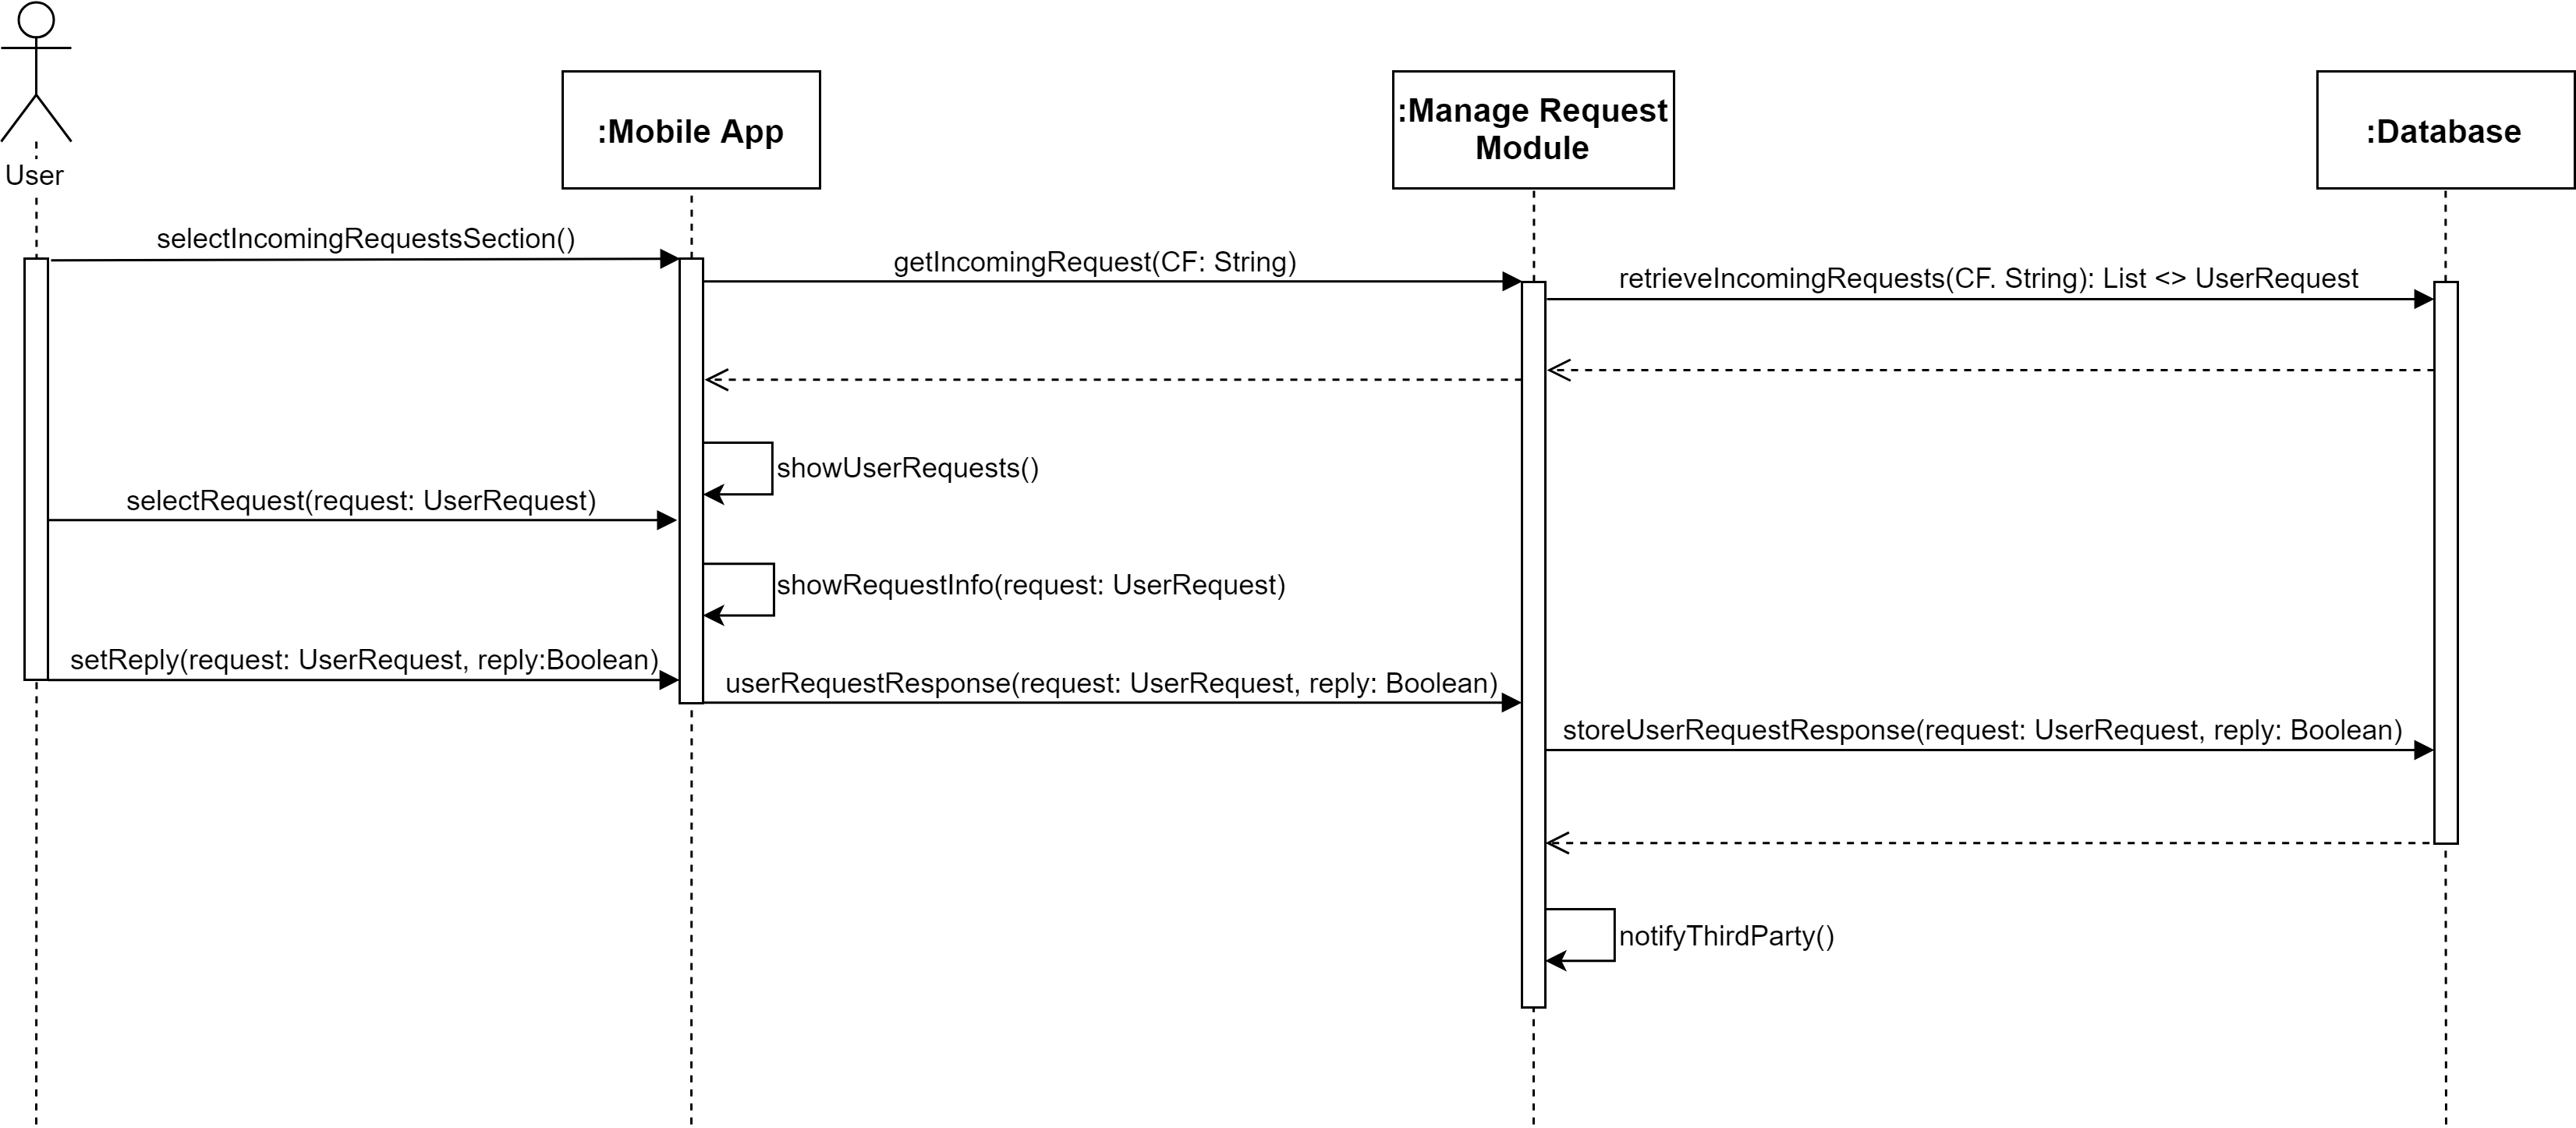
\includegraphics[scale=0.14]{./Pictures/acceptRequest.png}
    \caption{User acceptance of a request made by a Third Party}
    
\end{figure}

\subsection{Dispatch of a group subscription request}
A Third Party selects the New Request button with subscription mode, in the group section; it fills out the form with the kind of data it desires to receive, the characteristics on which the group research will be performed (age range, gender, location, weight and height range) and the update interval time. The Request Module retrieves the information from the database, creating a group with data that match the parameters selected, and checks if the number of individuals in this group is greater than 1000. If it is, the module makes the data anonymous by means of an anonymous identifier associated to each individual, and sends the data to the Third Party.

\begin{figure}[H]

    \centering
    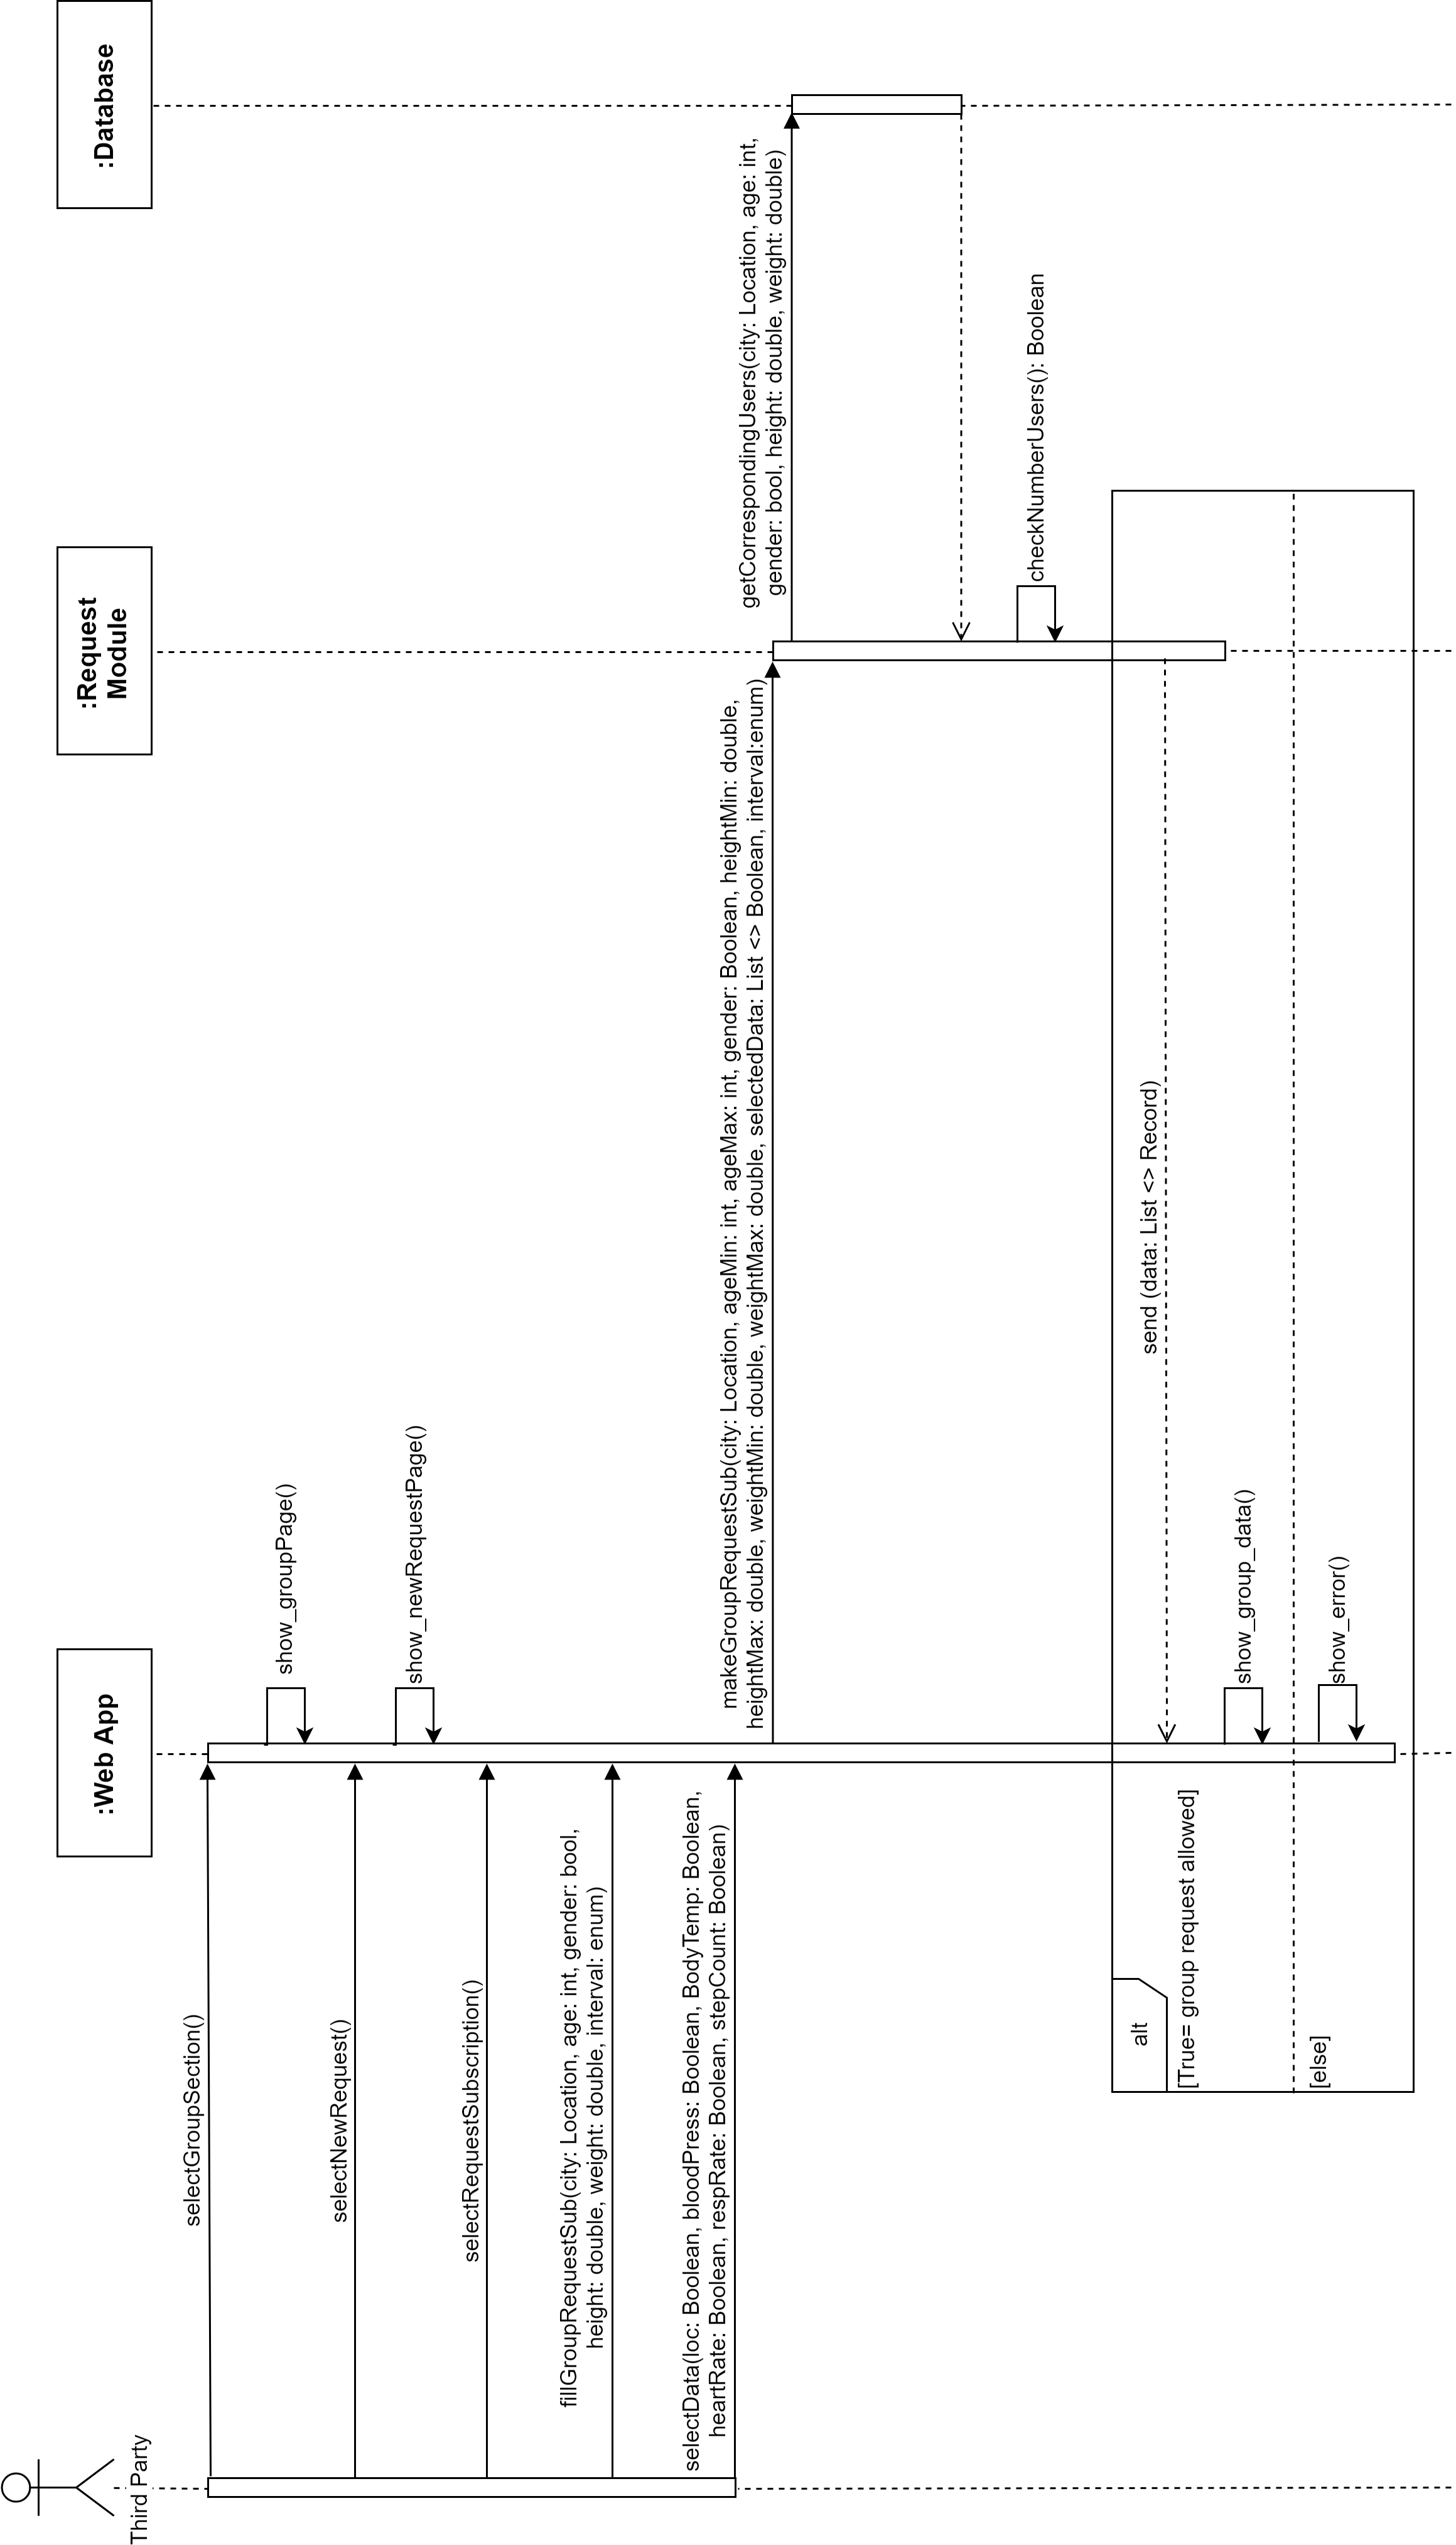
\includegraphics[scale=0.2]{./Pictures/groupRequestSeqDiagDDV.png}
    \caption{Group request by a Third Party}
    
\end{figure}

\subsection{Visualization of User data}
The Third Party can see the list of performed User requests, organized by status: Accepted, Refused or Pending. The Data Module retrieves the requests from the database and sends them to the client, taking only those of the selected status. Assuming that the Third Party is in the Accepted Requests section, now it can select the target request and the application shows the related records of the request.

\begin{figure}[H]

    \centering
    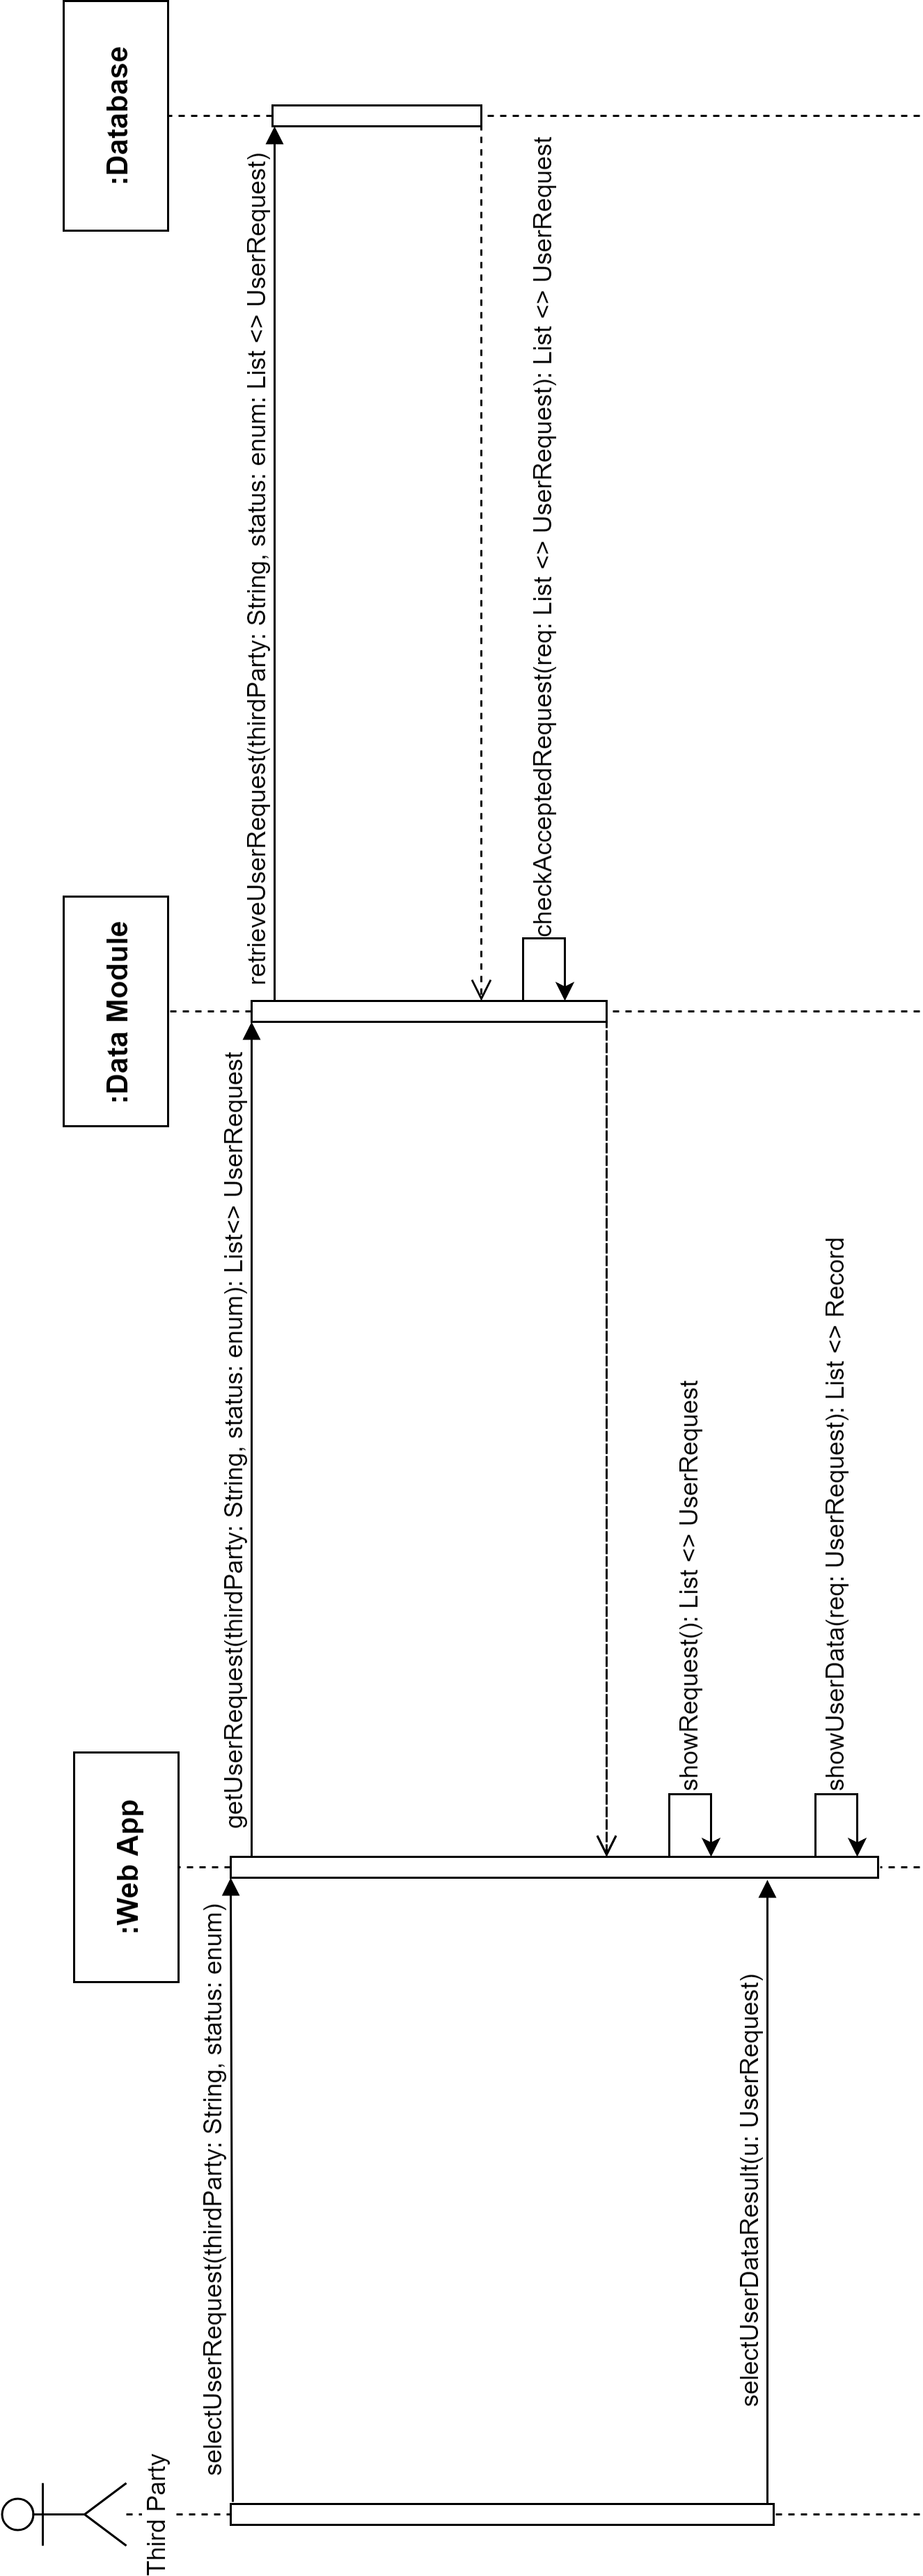
\includegraphics[scale=0.17]{./Pictures/showDataResultV.png}
    \caption{Visualization of data of a User that has already accepted the request}

\end{figure}

\subsection{Emergency}

The smart device collects parameters that exceed predeterminate thresholds: this is a signal of an emergency.
The User History Module receives the critical data, constructs a Record and, in case the User has enabled the AutomatedSOS service, forwards it to the AutomatedSOS Module to be analyzed in more detail.
The AutomatedSOS Module performs checks in order to identify if the data correspond to an emergency. If no critical parameters have been found, the module simply send the record back to the User History Module, after updating it with the correct emergency status (in this case false). If an emergency is actually detected, the AutomatedSOS Module proceeds to create a brief textual diagnosis of the health status. From the textual diagnosis, an audio diagnosis is generated with the use of the Festival Speech Synthesis System, an open source tool that offers a full text to speech system. At this point everything is ready for the call to the NHS through the CallHub external service. The same service is used to send a text message to the contacts specified by the user.
\begin{figure}[H]

    \centering
    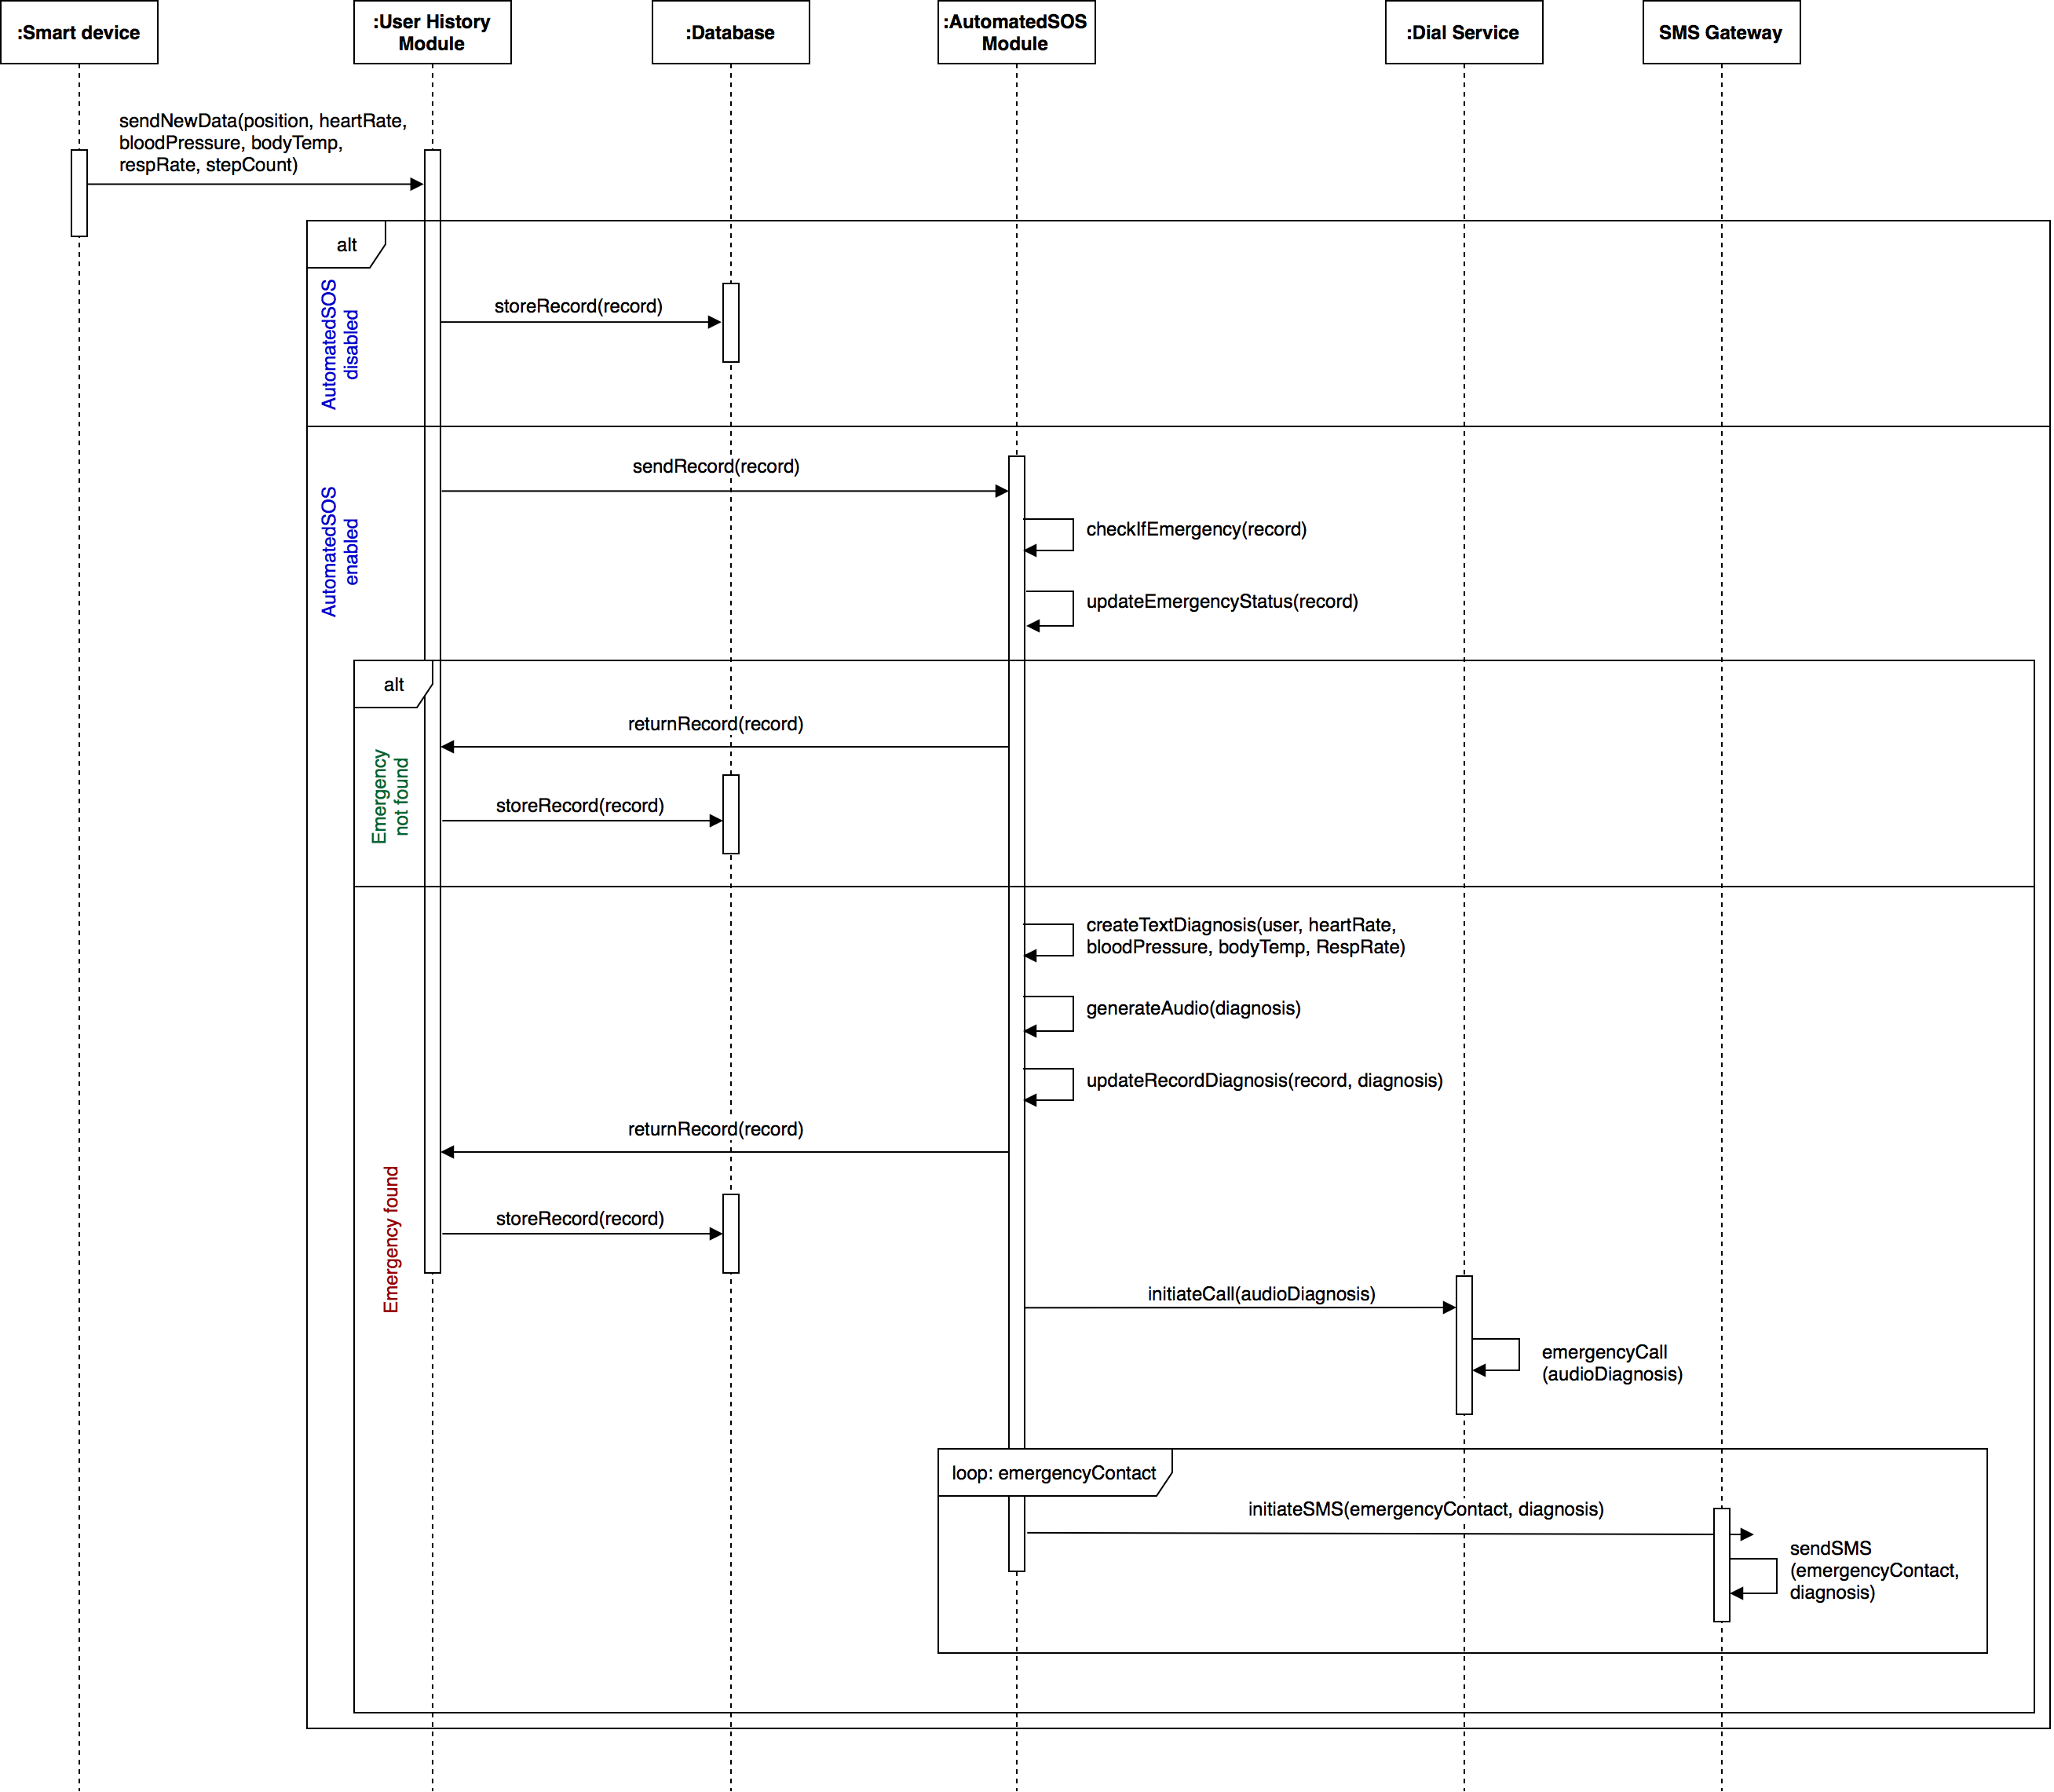
\includegraphics[scale=0.15]{./Pictures/sequence-emergency.png}
    \caption{Emergency management in AutomatedSOS}
    
\end{figure}

\subsection{Creation of a new run}
An Organizer creates a new run by filling out the form with all the details: day of the run, start time, starting point, ending point, list of intermediate points and maximum number of participants. The Track4Run Module defines the path that contains all the points selected by the Organizer through the map service and performs the checks to validate the run. If it is allowed, the module adds it to the list of scheduled run and the application shows a confirmation message to the Organizer. Otherwise, the application shows an error message.

\begin{figure}[H]

    \centering
    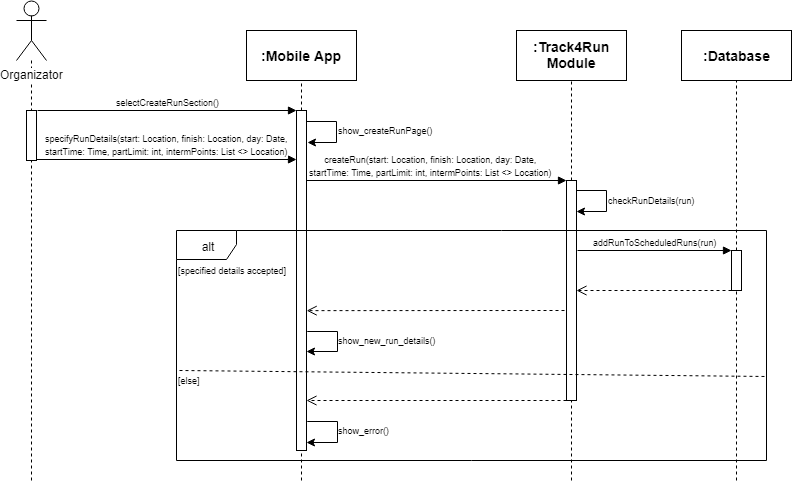
\includegraphics[scale=0.14]{./Pictures/createRunSeqDiagDD.png}
    \caption{Create a new run by an Organizer}
    
\end{figure}

\subsection{Enroll to a run}
Users can view the list of scheduled runs and perform a custom research by date, location and maximum number of participants. The Track4Run Module retrieves the matching runs from the database. Users can select a specific run and consult the details of the event. At this point he/she can decide to enroll to a run: the module checks if there are available entries and, in case of a positive response, the enrollment is allowed and the User is added to the list of participants of that run.

\begin{figure}[H]

    \centering
    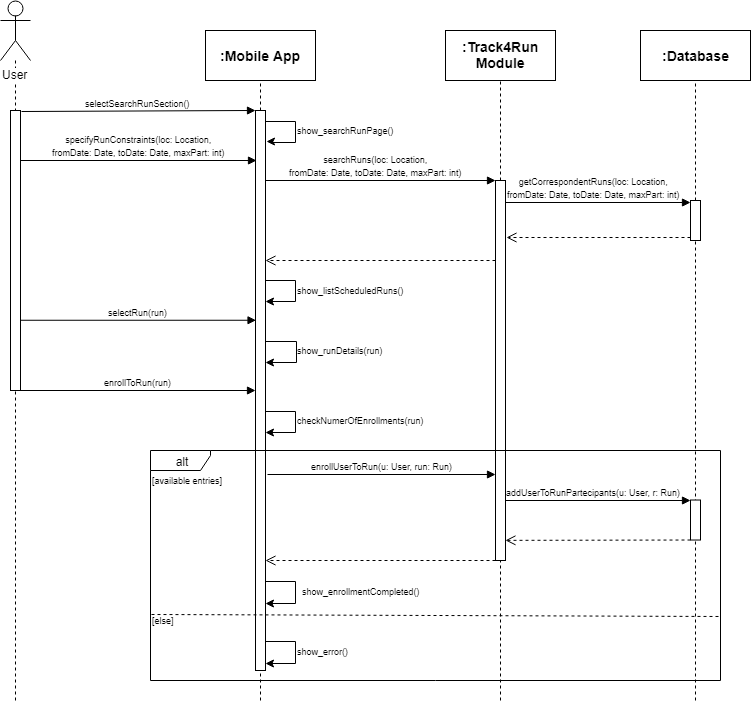
\includegraphics[scale=0.165]{./Pictures/enrollSeqDiagDD.png}
    \caption{Enrollment to a scheduled run by a User}
    
\end{figure}

\newpage